% Appendix B — H3X group 14-17 fan-out + group-16 sweet spot.
\section{Appendix B --- The $H_3X$ group-14--17 fan-out}
\label{app:B}

The binary $H_3X$ family is the campaign's primary search space. Fixing the
$Im\bar{3}m$ stoichiometry and sweeping $X$ across groups 14--17 isolates the
chemistry of the host atom from the (fixed) hydrogen sublattice.
Tab.~\ref{tab:fanout} is the converged fan-out; every $T_c$ carries a
\tierGreen\ verdict against Eq.~\eqref{eq:ad}.

\begin{table}[h]
\centering
\small
\begin{tabular}{llccccl}
\toprule
\textbf{Candidate} & \textbf{group} & \textbf{$\lambda_{\mathrm{BZ}}$} &
  \textbf{$\omega_{\log}$ (K)} & \textbf{$T_c$ (K)} & \textbf{stable?} &
  \textbf{note} \\
\midrule
\ce{H3Si} & 14 & 1.787 & 590  & 78  & \checkmark & stable, weak-$\lambda$ \\
\ce{H3O}  & 16 & 2.479 & 1097 & 180 & \textbf{no} ($16/16$ imag) & harmonic artifact \\
\ce{H3O}  & 16 & 0.52--1.48 & --- & 9--109 & \checkmark (SSCHA) & anharmonic collapse \\
\ce{H3F}  & 17 & 0.807 & 659  & 31  & \checkmark & stable, weak-$\lambda$ \\
\ce{H3Cl} & 17 & 1.43  & 1173 & 128 & \checkmark & stable, $\omega$-capped \\
\ce{H3Br} & 17 & 4.42  & 531  & 110 & \checkmark ($16/16$) & strong-$\lambda$, $\omega$-bottleneck \\
\ce{H3Br} & 17 & 2.156 & 1046 & \textbf{158} & \checkmark ($8/8$) & 200 GPa record (Apx.~\ref{app:F}) \\
\ce{H3Po} & 16 & 3.05  & 265  & 48  & \textbf{no} (soft) & heavy-$X$ double fail \\
\bottomrule
\end{tabular}
\caption{$H_3X$ fan-out across groups 14--17 ($\mu^\ast = 0.10$,
$Im\bar{3}m$ unless noted). Two distinct \ce{H3Br} state points appear: the
strong-$\lambda$ low-pressure branch ($\lambda=4.42$, $\omega_{\log}=531$)
and the high-$\omega$ \SI{200}{\giga\pascal} record (Apx.~\ref{app:F}). Every
row is reproduced to libm precision.}
\label{tab:fanout}
\end{table}

\begin{figure}[h]
\centering
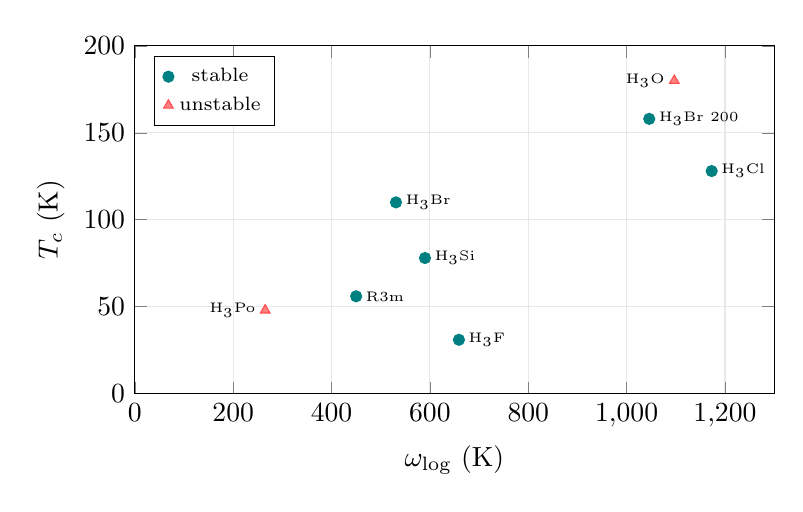
\begin{tikzpicture}
\begin{axis}[
  width=0.80\linewidth, height=6cm,
  xlabel={$\omega_{\log}$ (K)}, ylabel={$T_c$ (K)},
  xmin=0, xmax=1300, ymin=0, ymax=200,
  grid=both, grid style={gray!18},
  legend pos=north west, legend style={font=\scriptsize},
]
\addplot[only marks,mark=*,draw=teal,fill=teal,
  nodes near coords,point meta=explicit symbolic,
  every node near coord/.append style={font=\tiny,anchor=west}]
  coordinates {
    (590,78)[H$_3$Si] (659,31)[H$_3$F] (1173,128)[H$_3$Cl]
    (531,110)[H$_3$Br] (450,56)[R3m] (1046,158)[H$_3$Br 200] };
\addlegendentry{stable}
\addplot[only marks,mark=triangle*,draw=red!70,fill=red!50,
  nodes near coords,point meta=explicit symbolic,
  every node near coord/.append style={font=\tiny,anchor=east}]
  coordinates { (1097,180)[H$_3$O] (265,48)[H$_3$Po] };
\addlegendentry{unstable}
\end{axis}
\end{tikzpicture}
\caption{$H_3X$ fan-out: $T_c$ versus $\omega_{\log}$. Stable candidates
(teal) cluster along an $\omega_{\log}$-limited envelope; the highest-$T_c$
points (\ce{H3O}, \ce{H3Po}, red) are dynamically unstable. \ce{H3Br} at
\SI{200}{\giga\pascal} ($\omega_{\log}=\SI{1046}{\kelvin}$,
$T_c=\SI{158}{\kelvin}$) is the stable frontier.}
\label{fig:fanout-scatter}
\end{figure}

\paragraph{Verbatim verdicts (g5).}
\begin{lstlisting}[basicstyle=\ttfamily\footnotesize,frame=single,xleftmargin=0pt]
$ hexa verify --expr allen_dynes_tc 1.787 590.1 0.10 78.18 --tol 0.01
  calc=78.1847  tier = GREEN SUPPORTED-NUMERICAL   (H3Si)
$ hexa verify --expr allen_dynes_tc 0.807 658.6 0.10 31.41 --tol 0.01
  calc=31.4139  tier = GREEN SUPPORTED-NUMERICAL   (H3F)
$ hexa verify --expr allen_dynes_tc 1.43  1173  0.10 127.63 --tol 0.01
  calc=127.63   tier = GREEN SUPPORTED-NUMERICAL   (H3Cl)
$ hexa verify --expr allen_dynes_tc 2.479 1096.6 0.10 179.78 --tol 0.01
  calc=179.779  tier = GREEN SUPPORTED-NUMERICAL   (H3O harmonic = artifact)
\end{lstlisting}

\paragraph{Group-16 sweet spot, with a caveat.}
The group-16 hosts (\ce{H3O}, \ce{H3Po}) carry the campaign's largest
\emph{harmonic} couplings ($\lambda = 2.48$, $3.05$) and the highest extrapolated
$T_c$ --- but both are dynamically unstable. Group-16 is a coupling sweet
spot and a stability trap simultaneously. The lighter group-17 \ce{H3Cl}
($\omega_{\log} = \SI{1173}{\kelvin}$) is the best \emph{stable} binary at
moderate pressure, but its coupling is capped near $\lambda = 1.4$. This
splitting --- strong coupling \emph{or} stability, never both --- is the
empirical signature of the N5 wall, quantified in Appendix~\ref{app:D}.
